\documentclass[12pt]{ctexart}
\usepackage{amsmath} % 用于数学公式
\usepackage{graphicx} % 用于插入图片
\usepackage{listings} % 用于插入代码
\usepackage{float}    % 用于控制图表浮动位置

\usepackage{booktabs} % 用于创建更美观的三线表
\usepackage{siunitx}  % 用于标准地排版物理单位和数值
\usepackage{amsmath}  % 用于数学公式环境
\sisetup{per-mode=symbol} % 设置单位格式，例如 m/s

\usepackage{fancyhdr}   % 用于自定义页眉页脚
\usepackage{caption}   % 用于自定义图表标题
\usepackage{subcaption} % 用于子图环境
\usepackage{hyperref}  % 用于创建超链接
\usepackage{makecell}
\usepackage{multirow}  

% \pdfcompresslevel=9

\graphicspath{{./figures/}}

\usepackage[left=2.5cm, right=2.5cm, top=2cm, bottom=2cm]{geometry}

% \setlength{\jot}{6pt} % 增加多行公式之间的行距

\linespread{1.5}

\pagestyle{fancy}

\begin{document}

% \maketitle
\thispagestyle{empty}

\begin{figure}[t]
    \centering
    
\includegraphics[width=13cm]{./figures/logo1.png}
\end{figure}

\vspace*{\fill}
    \begin{center}
        \Huge\textbf{实验3：连续时间系统模拟}
    \end{center}
\vspace*{\fill}

\begin{table}[H]
    \centering
    \large
    \begin{tabular}{ll}
    \textbf{课程:} & 信号与系统实验 \\
    \textbf{姓名:} & 郭浩然 \\
    \textbf{学号:} & 2024303980 \\
    \textbf{桌号:} & 18 \\
    \textbf{班级:} & 10班 \\
    \textbf{学院:} & 民航学院 \\
    \textbf{专业:} & 飞行器控制与信息工程 \\
    \textbf{时间:} & \today \\
    \end{tabular}
\end{table}

\newpage

\tableofcontents
\newpage

% ===================================================================
% 报告正文开始
% 请将此部分代码粘贴到您的 \tableofcontents 和 \newpage 之后
% ===================================================================

\section{实验目的}
\begin{enumerate}
    \item 了解基本运算器——比例放大器、加法器和积分器的电路结构和运算功能。
    \item 掌握用基本运算单元模拟连续时间一阶系统原理与测试方法。
\end{enumerate}

\section{实验器材}
\begin{enumerate}
    \item 双踪示波器 1台
    \item 数字万用表 1块
    \item 电压表及直流信号源模块 S1 1块
    \item 信号源及频率计模块 S2 1块
    \item 基本运算单元与连续系统模块 S9 1块
\end{enumerate}

\section{实验原理}

\subsection{线性系统的模拟}
系统的模拟就是用由基本运算单元组成的模拟装置来模拟实际的系统。这些实际系统可以是电的或非电的物理量系统，也可以是社会、经济和军事等非物理量系统。模拟装置可以与实际系统的内容完全不同，但是两者的微分方程完全相同，输入、输出关系即传输函数也完全相同。模拟装置的激励和响应是电物理量而实际系统的激励和响应不一定是电物理量，但它们之间的关系是一一对应的。所以，可以通过对模拟装置的研究来分析实际系统，最终达到一定条件下确定最佳参数的目的。

本实验所说的系统的模拟就是由基本的运算单元(放大器、加法器，积分器等)组成的模拟装置，来模拟实际系统的传输特性。

\subsection{三种基本运算电路}
\subsubsection{比例放大器}
电路如图\ref{fig:op-amp-prop}所示，其输入输出关系为：
\[ u_{0} = -\frac{R_{2}}{R_{1}} \cdot u_{1} \]

\begin{figure}[H]
    \centering
    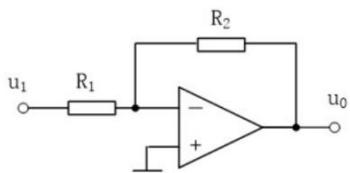
\includegraphics[width=0.4\textwidth]{figures/fig3-1.png}
    \caption{比例放大电路连线示意图}
    \label{fig:op-amp-prop}
\end{figure}

\subsubsection{加法器}
电路如图\ref{fig:op-amp-add}所示，其输入输出关系为：
\[ u_{0} = -\frac{R_{2}}{R_{1}} (u_{1} + u_{2}) \]
当 $R_{1} = R_{2}$ 时，上式简化为 $u_{0} = -(u_{1} + u_{2})$。

\begin{figure}[H]
    \centering
    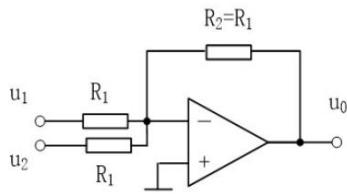
\includegraphics[width=0.4\textwidth]{figures/fig3-2.png}
    \caption{加法器电路连线示意图}
    \label{fig:op-amp-add}
\end{figure}

\subsubsection{积分器}
电路如图\ref{fig:op-amp-int}所示，其输入输出关系为：
\[ u_{2} = -\frac{1}{RC}\int_{-\infty}^{t}u_{1}(\tau)d\tau \]

\begin{figure}[H]
    \centering
    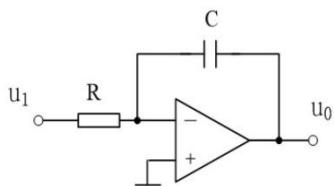
\includegraphics[width=0.4\textwidth]{figures/fig3-3.png}
    \caption{积分器电路连接示意图}
    \label{fig:op-amp-int}
\end{figure}

\subsection{一阶系统的模拟}
一阶RC电路如图\ref{fig:rc-circuit}(a)所示，可用以下微分方程描述：
\[ \frac{\mathrm{d}y(t)}{\mathrm{d}t} + \frac{1}{RC} y(t) = \frac{1}{RC} x(t) \]
其模拟框图如图\ref{fig:rc-circuit}(b)和(c)所示，两者在数学关系上是等效的。对应的一阶系统模拟实验电路如图\ref{fig:rc-circuit}(d)所示。

\begin{figure}[H]
    \centering
    \begin{subfigure}[b]{0.38\textwidth}
        \centering
        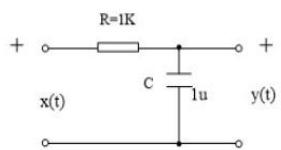
\includegraphics[width=\textwidth]{figures/fig3-4a.png}
        \caption{一阶RC电路}
    \end{subfigure}
    \hfill
    \begin{subfigure}[b]{0.38\textwidth}
        \centering
        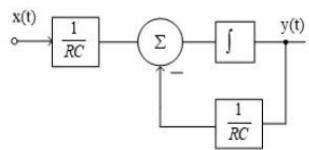
\includegraphics[width=\textwidth]{figures/fig3-4b.png}
        \caption{模拟框图1}
    \end{subfigure}
    
    \vspace{1em} % 增加垂直间距
    
    \begin{subfigure}[b]{0.38\textwidth}
        \centering
        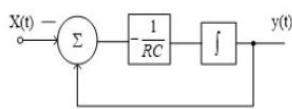
\includegraphics[width=\textwidth]{figures/fig3-4c.png}
        \caption{模拟框图2 (等效)}
    \end{subfigure}
    \hfill
    \begin{subfigure}[b]{0.38\textwidth}
        \centering
        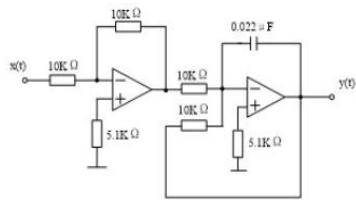
\includegraphics[width=\textwidth]{figures/fig3-4d.png}
        \caption{一阶系统模拟实验电路}
    \end{subfigure}
    \caption{一阶RC电路及其模拟}
    \label{fig:rc-circuit}
\end{figure}

\newpage % 避免步骤和原理挤在一起，可根据需要移除

\section{实验步骤}
\subsection{任务一：基本运算器——加法器的观测}
\begin{enumerate}
    \item 模块关电，按如图\ref{fig:adder-exp-circuit}所示连接实验电路。
    \item 将模块S1的直流输出1(P1)和直流输出2(P2)分别接至加法器的 $u_{1}$ 和 $u_{2}$。模块开电，适当调节S1模块中的W1、W2，并记录P1和P2的电压值。
    \item 用万用表测量输出 $u_{0}$ 端电压。验证在反相加法器中，输出电压是否为两路输入电压之和取反相，完成表\ref{tab:adder-data}的记录。
    \item 将输入一改为峰峰值为 \SI{2}{\volt}、频率为 \SI{500}{\hertz} 的正弦波(方波)，再观察输入及输出波形，并完成记录。
\end{enumerate}

\begin{figure}[H]
    \centering
    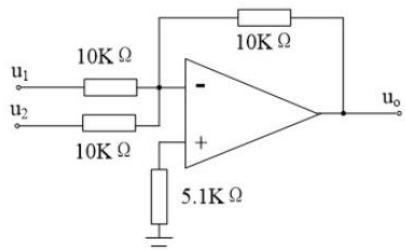
\includegraphics[width=0.4\textwidth]{figures/fig3-6.png}
    \caption{加法器实验电路图}
    \label{fig:adder-exp-circuit}
\end{figure}

\subsection{任务二：基本运算器——比例放大器的观测}
\begin{enumerate}
    \item 模块关电，连接如图\ref{fig:prop-exp-circuit}所示实验电路。$R_1, R_2$可选择2组不同的电阻值以改变放大比例。
    \item 模块开电，信号发生器或模块产生幅度为 \SI{1}{\volt}、频率为 \SI{1}{\kilo\hertz} 的正弦波送入输入端，示波器同时观察并比较输入、输出波形，完成表\ref{tab:prop-data}的记录。
\end{enumerate}

\begin{figure}[H]
    \centering
    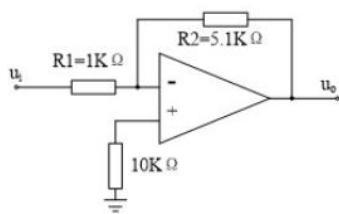
\includegraphics[width=0.4\textwidth]{figures/fig3-7.png}
    \caption{比例放大器实验电路图}
    \label{fig:prop-exp-circuit}
\end{figure}

\subsection{任务三：基本运算器——积分器的观测}
为了防止低频信号增益过大，在电容两端并了一个 \SI{20}{\kilo\ohm} 电阻加以限制，同相输入端的 \SI{10}{\kilo\ohm} 电阻起到平衡电阻的作用。其输入输出关系为：
\[ u_{0}(t) = - \frac{1}{RC} \int_{t_{0}}^{t} u_{i}(\tau) \mathrm{d}\tau + u_{0}(t_{0}) \]
\begin{enumerate}
    \item 模块关电，连接如图\ref{fig:int-exp-circuit}所示实验电路。（\SI{20}{\kilo\ohm} 的电阻，可用两个 \SI{10}{\kilo\ohm} 的电路串联代替。）
    \item 模块开电，信号发生器或模块S2产生 $f = \SI{1}{\kilo\hertz}$ 的方波送入输入端，示波器同时观察输入、输出波形并比较自行完成实验数据记录。
\end{enumerate}

\begin{figure}[H]
    \centering
    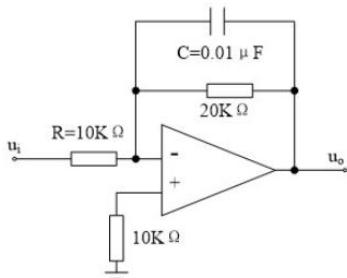
\includegraphics[width=0.3\textwidth]{figures/fig3-8.png}
    \caption{积分器实验电路图}
    \label{fig:int-exp-circuit}
\end{figure}

\subsection{任务四：一阶RC电路的模拟}
图\ref{fig:rc-circuit}(a)为一阶RC电路，模块关电，按图\ref{fig:rc-circuit}(d)所示连接其一阶模拟电路。(阻容元件根据需要进行选择，\SI{0.022}{\micro\farad} 电容可由两个 \SI{0.01}{\micro\farad} 电容并联代替)。模块开电，将信号发生器产生的幅度为\SI{2}{\volt}、频率 \SI{1}{\kilo\hertz} 的方波送入一阶模拟电路输入端，用示波器观测输出电压波形，验证其模拟情况。

\begin{figure}[H]
    \centering
    \begin{subfigure}{0.48\textwidth}
        \centering
        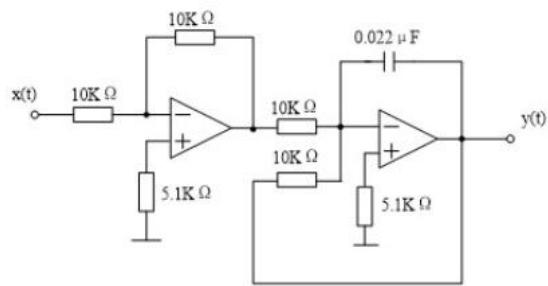
\includegraphics[width=\textwidth]{figures/fig3-9a.png}
        \caption{模块实验电路图1}
    \end{subfigure}
    \hfill
    \begin{subfigure}{0.48\textwidth}
        \centering
        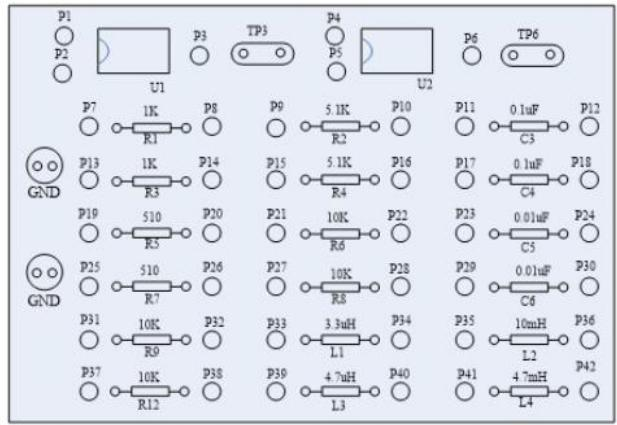
\includegraphics[width=\textwidth]{figures/fig3-9b.png}
        \caption{模块实验电路图2}
    \end{subfigure}
    \caption{模块实验电路图}
    \label{fig:module-circuit}
\end{figure}

\section{实验数据}
\subsection{照片记录各基本运算器输入输出波形}

\subsubsection{加法器}

% 开启一个浮动体环境，用来包裹左右两部分
\begin{figure}[H]
    \centering
    
    % --- 左侧：表格 ---
    % 宽度设为页面宽度的 0.48 (预留中间间隙)
    % [c] 表示垂直居中对齐
    \begin{minipage}[c]{0.48\textwidth}
        \centering
        % 注意：这里使用 \captionof{table} 而不是 simple \caption
        \captionof{table}{加法器直流输入测试数据}
        \label{tab:adder-data}
        % 将表格宽度设为 \linewidth 以自适应 minipage 宽度，或者保持原样
        \begin{tabular}{ccc}
            \toprule
            输入一 (\si{\volt}) & 输入二 (\si{\volt}) & 输出 (\si{\volt}) \\
            \midrule
            -2.2  & -2.73 & 4.94  \\
            2.00 & 5.08 & -7.07  \\
            1.66  & 1.03  & -2.7  \\
            \bottomrule
        \end{tabular}
    \end{minipage}
    \hfill % \hfill 负责在两个 minipage 之间撑开距离
    % --- 右侧：图片 ---
    \begin{minipage}[c]{0.48\textwidth}
        \centering
        % 图片宽度设为 \linewidth，即占满当前 minipage 的宽度
        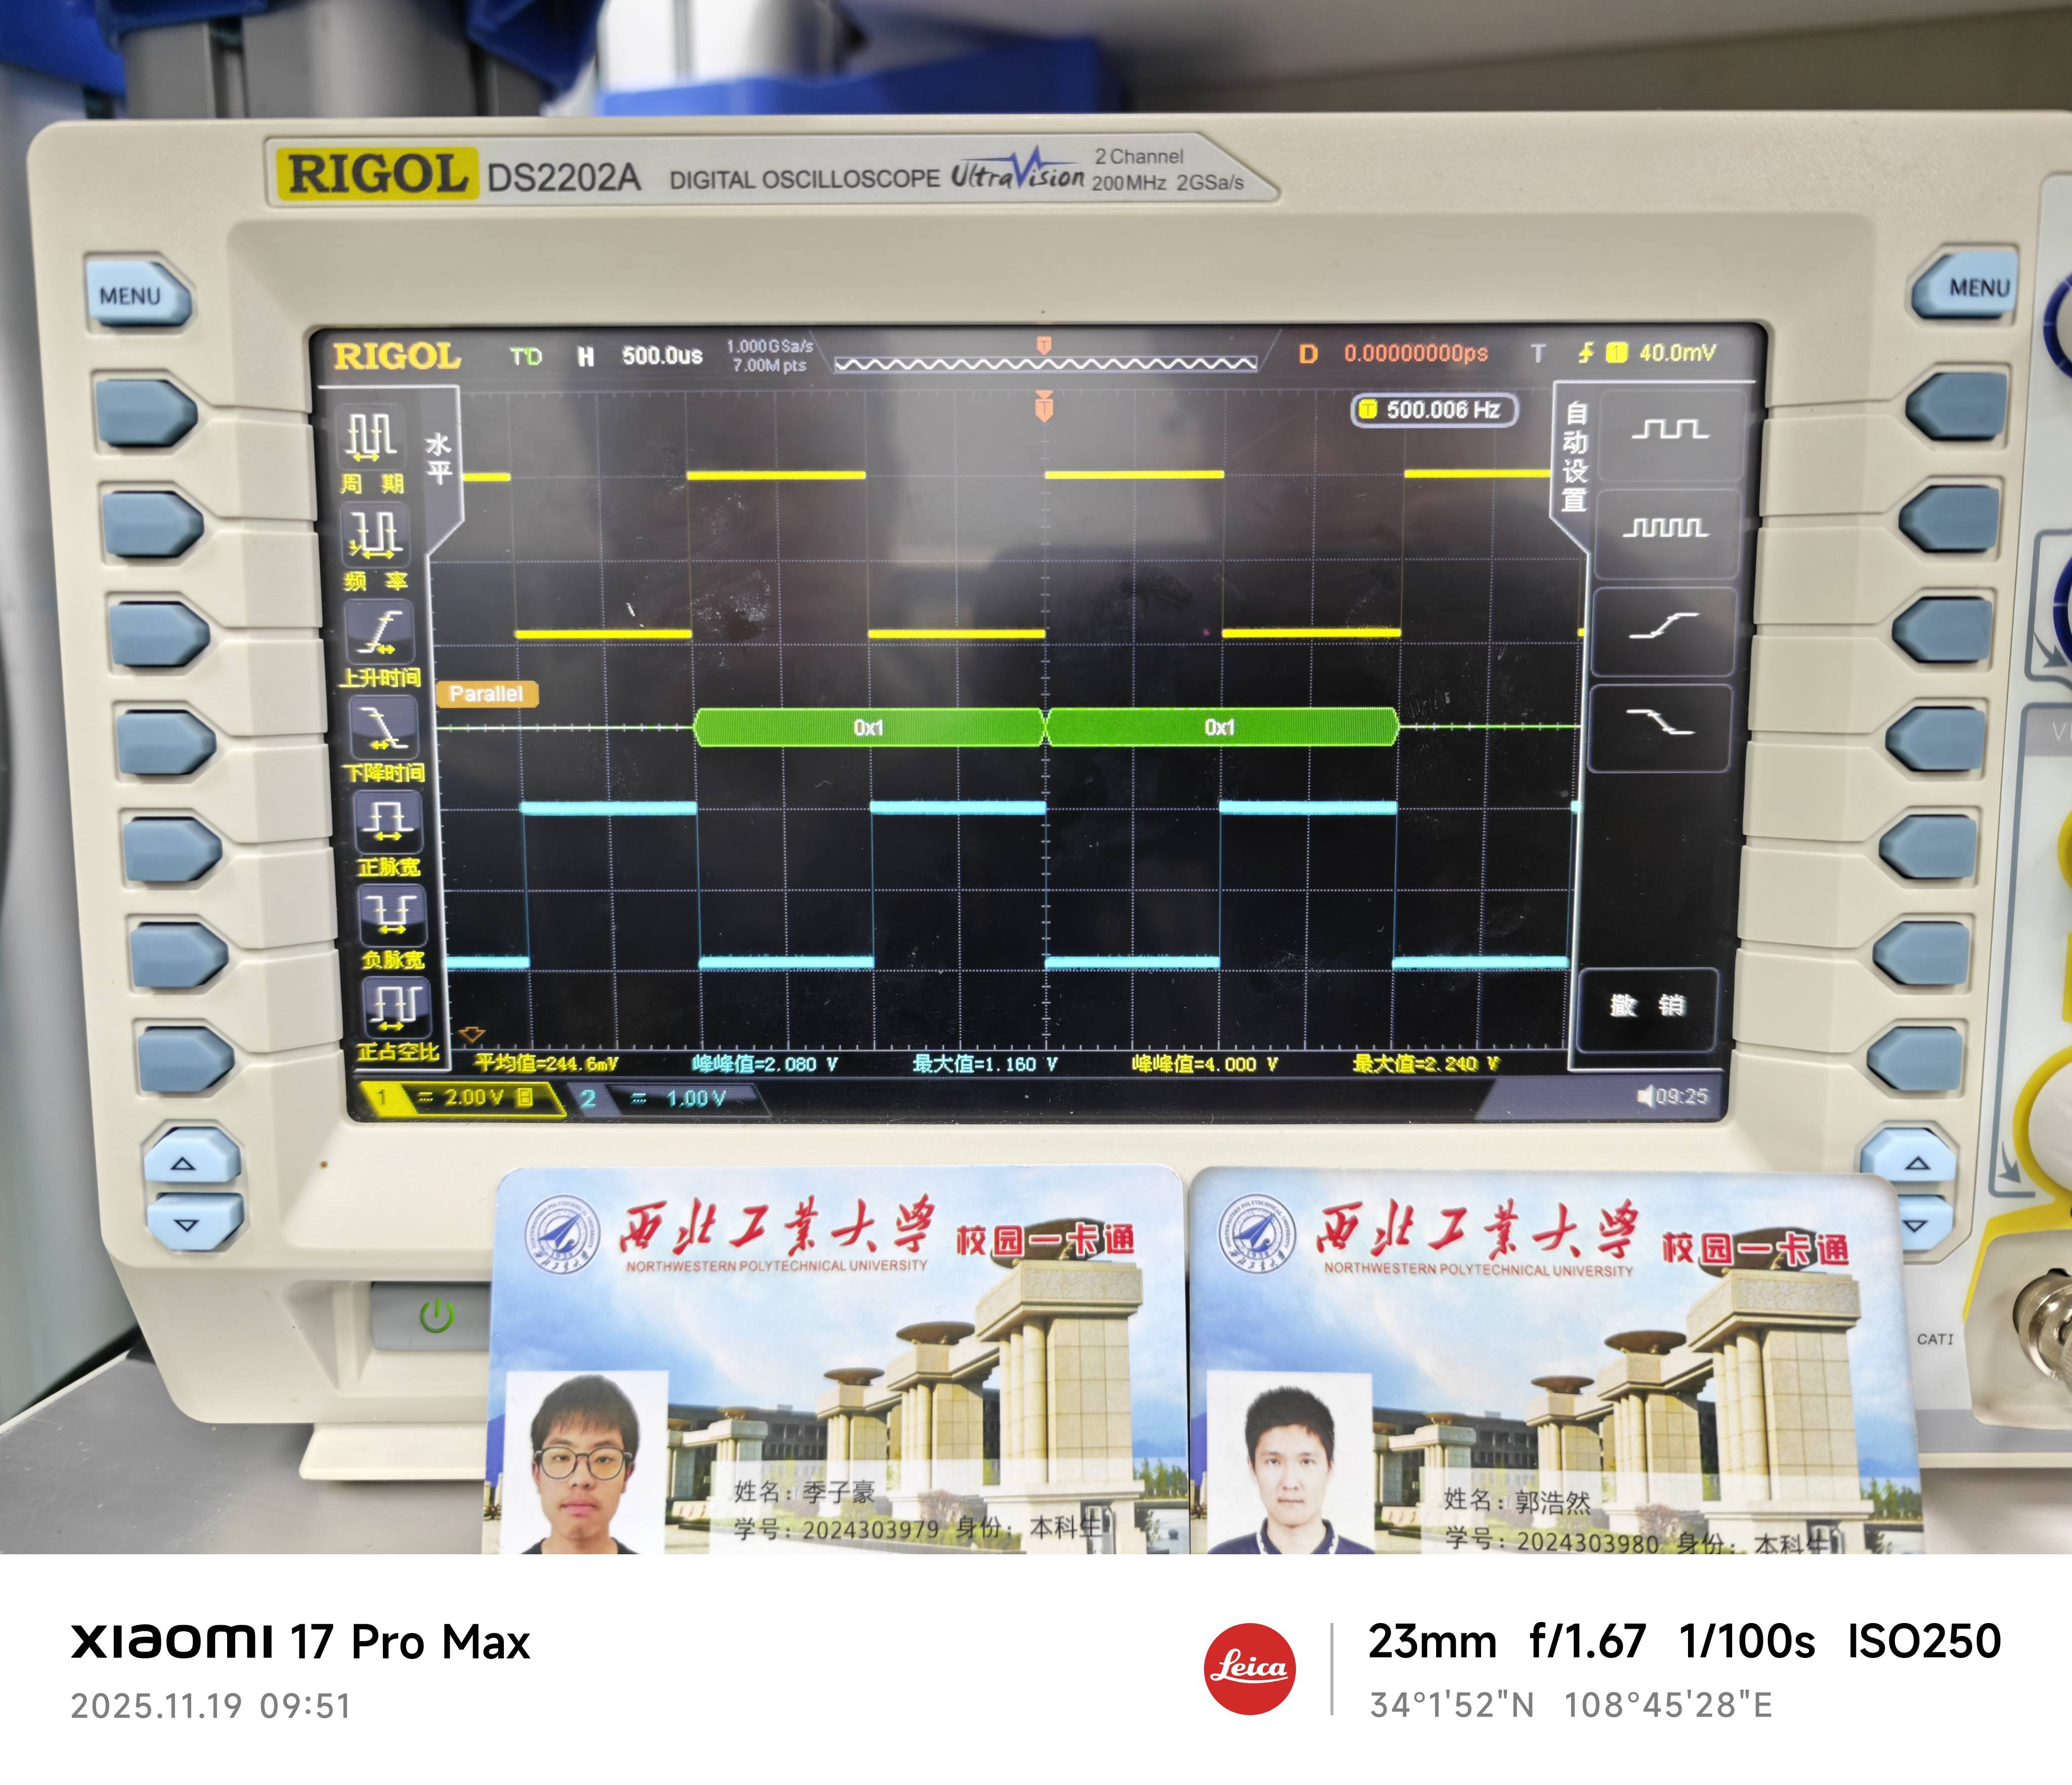
\includegraphics[width=\linewidth]{figures/反相加法器.jpg}
        \caption{加法器混合输入波形}
        \label{fig:result-adder}
    \end{minipage}
\end{figure}

由表\ref{tab:adder-data}可知：输出电压大致等于两路输入电压之和取反相，验证了加法器的功能。

当输入一改为峰峰值为 \SI{2}{\volt}、频率为 \SI{500}{\hertz} 的方波时，波形如图\ref{fig:result-adder}所示。从图中可以看出，加法器实现了对输入方波的直流偏置与反相。

\subsubsection{比例放大器}
测得实验数据如表\ref{tab:prop-data}所示。对应的示波器波形如图\ref{fig:result-prop}所示。

\begin{table}[H]
    \centering
    \caption{比例放大器测试数据}
    \label{tab:prop-data}
    \begin{tabular}{ccccc}
        \toprule
        组号 & 电阻 & 输入电压 & 输入波形 & 输出电压 (\si{\volt}) \\
        \midrule
        1 & $R_1 = \SI{1}{\kilo\ohm},\; R_2 = \SI{5.1}{\kilo\ohm}$ & \SI{1.000}{\volt} & \SI{1}{\kilo\hertz} 正弦波 & \SI{4.560}{\volt} \\
        2 & $R_1 = \SI{1}{\kilo\ohm},\; R_2 = \SI{10}{\kilo\ohm}$  & \SI{980.0}{\milli\volt} & \SI{1}{\kilo\hertz} 正弦波 & \SI{9.200}{\volt} \\
        \bottomrule
    \end{tabular}
\end{table}


\begin{figure}[H]
    \centering
    % 这里是您提到的，为两组数据分别提供照片的地方
    % 我使用了子图环境，请您准备两张照片
    \begin{subfigure}{0.48\textwidth}
        \centering
        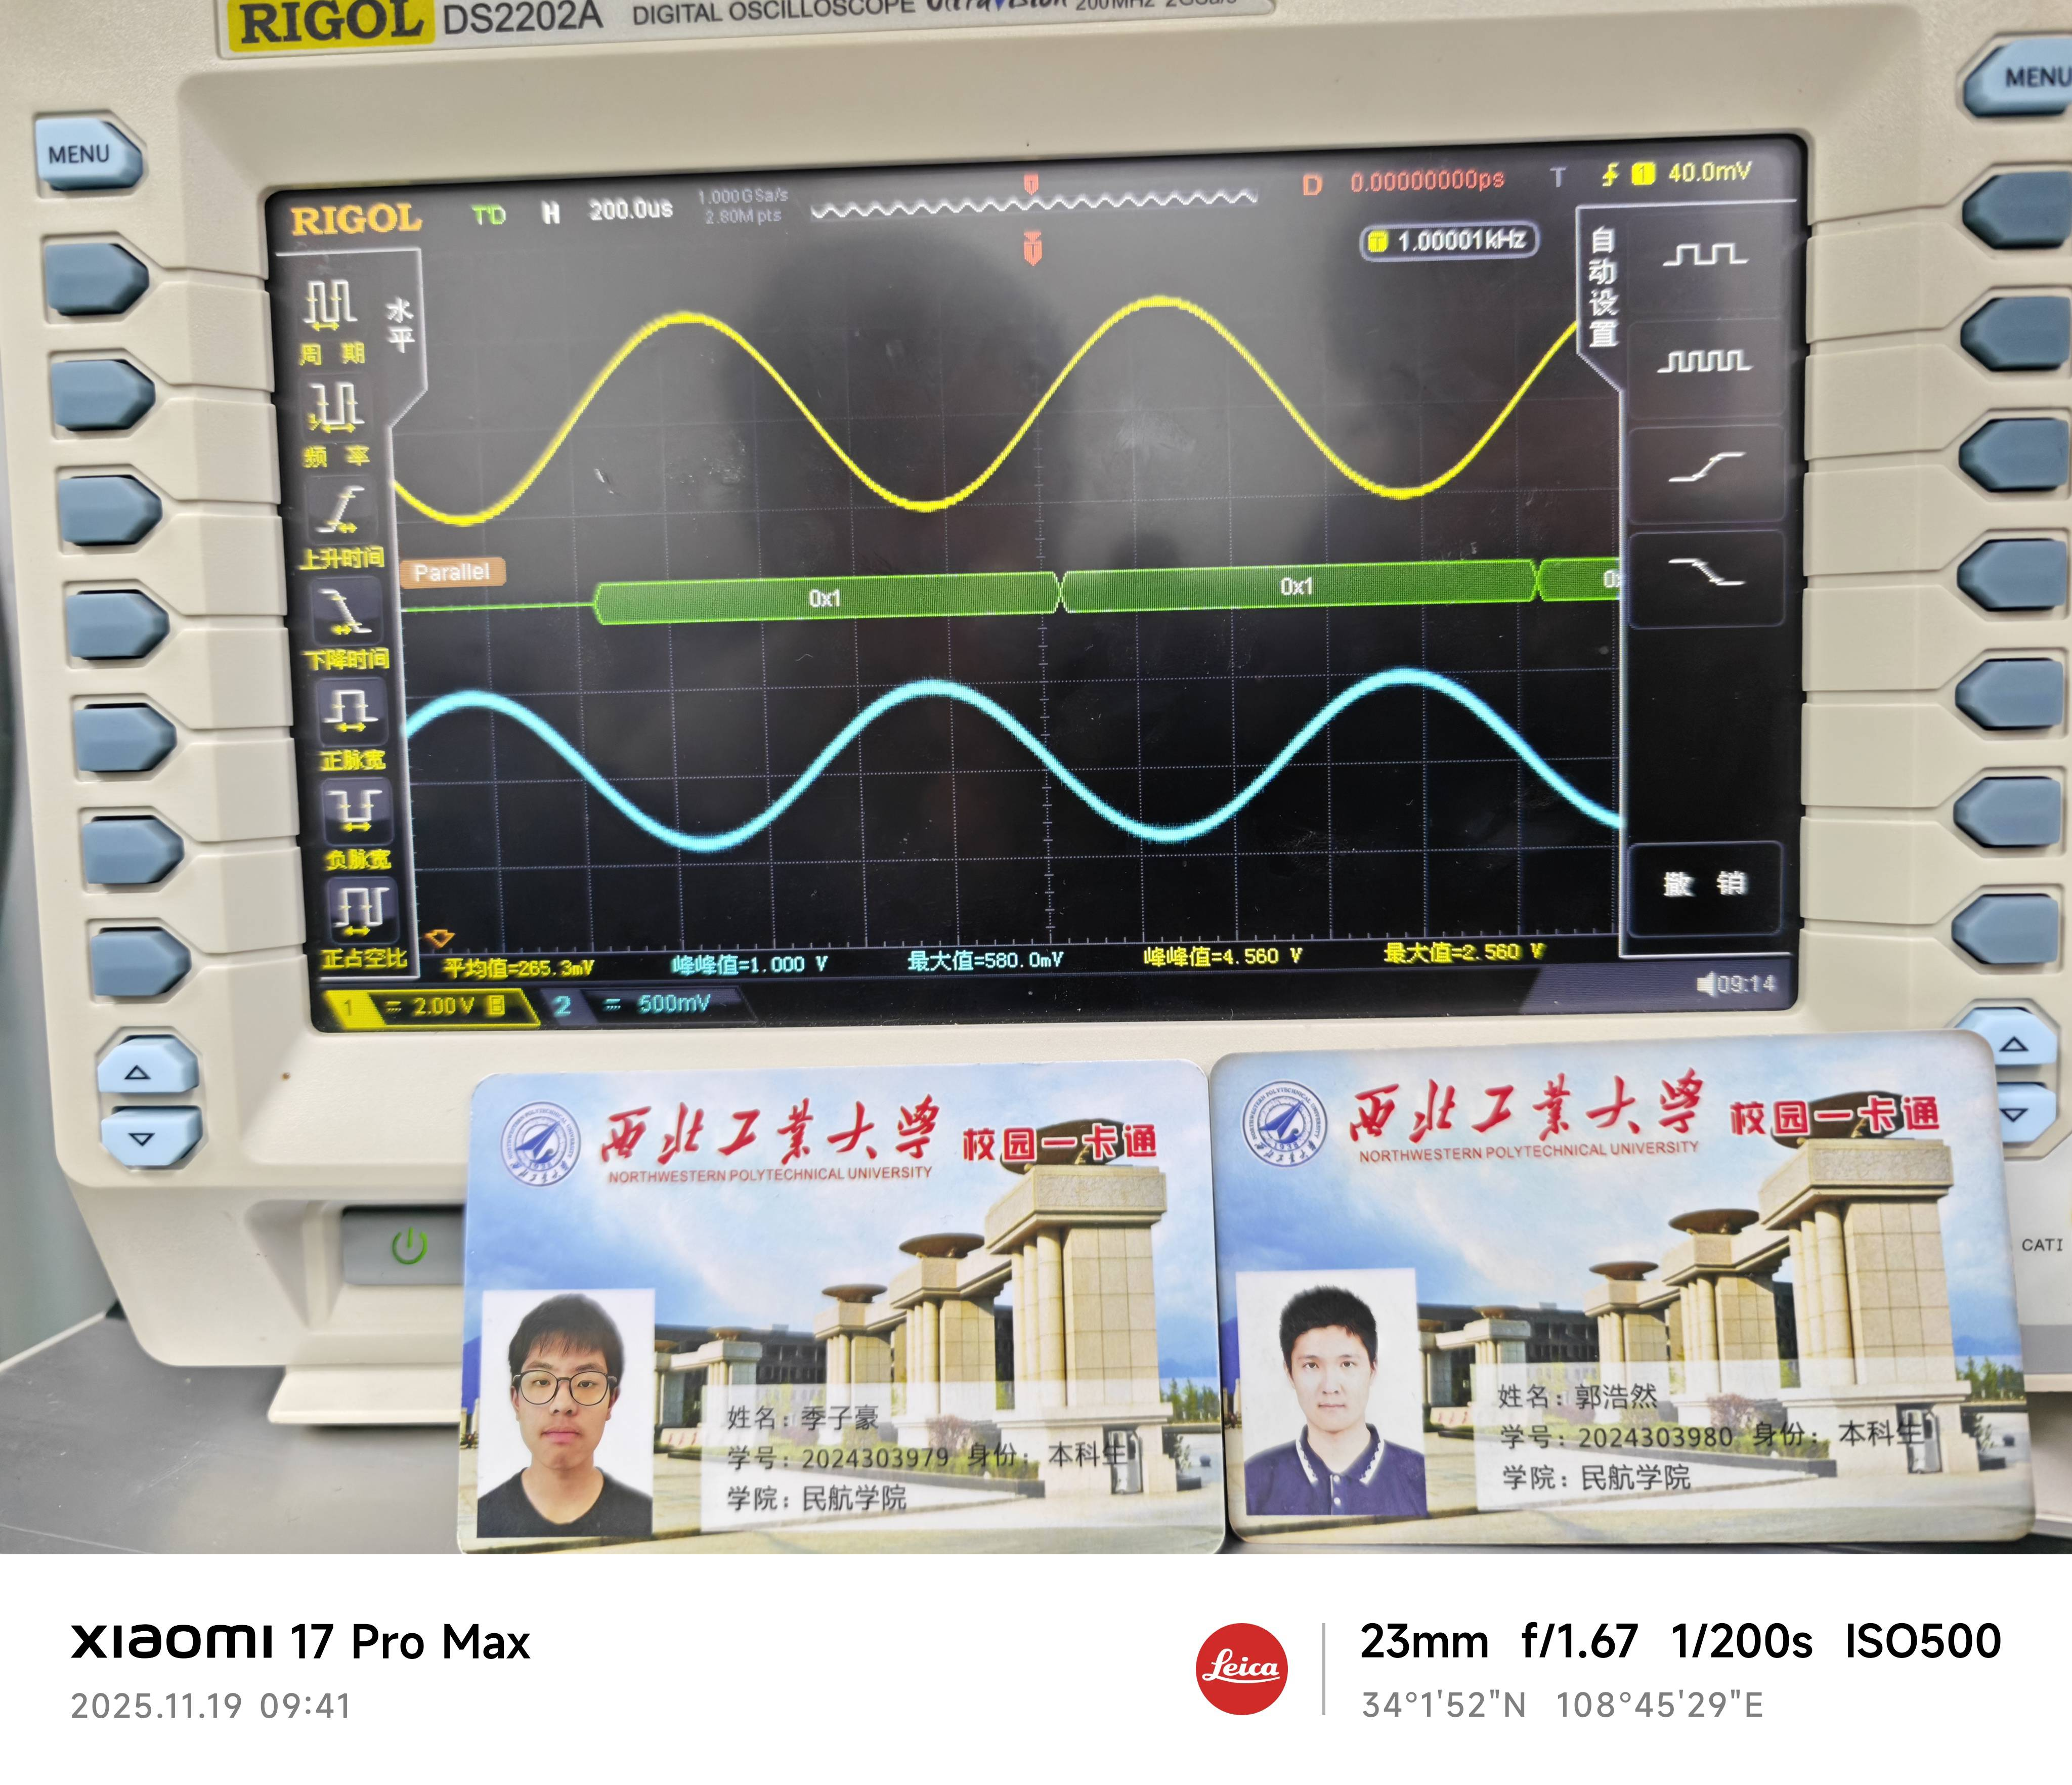
\includegraphics[width=\textwidth]{figures/比例器2.jpg}
        \caption{第一组电阻 ($R_2 = \SI{5.1}{\kilo\ohm}$)}
    \end{subfigure}
    \hfill
    \begin{subfigure}{0.48\textwidth}
        \centering
        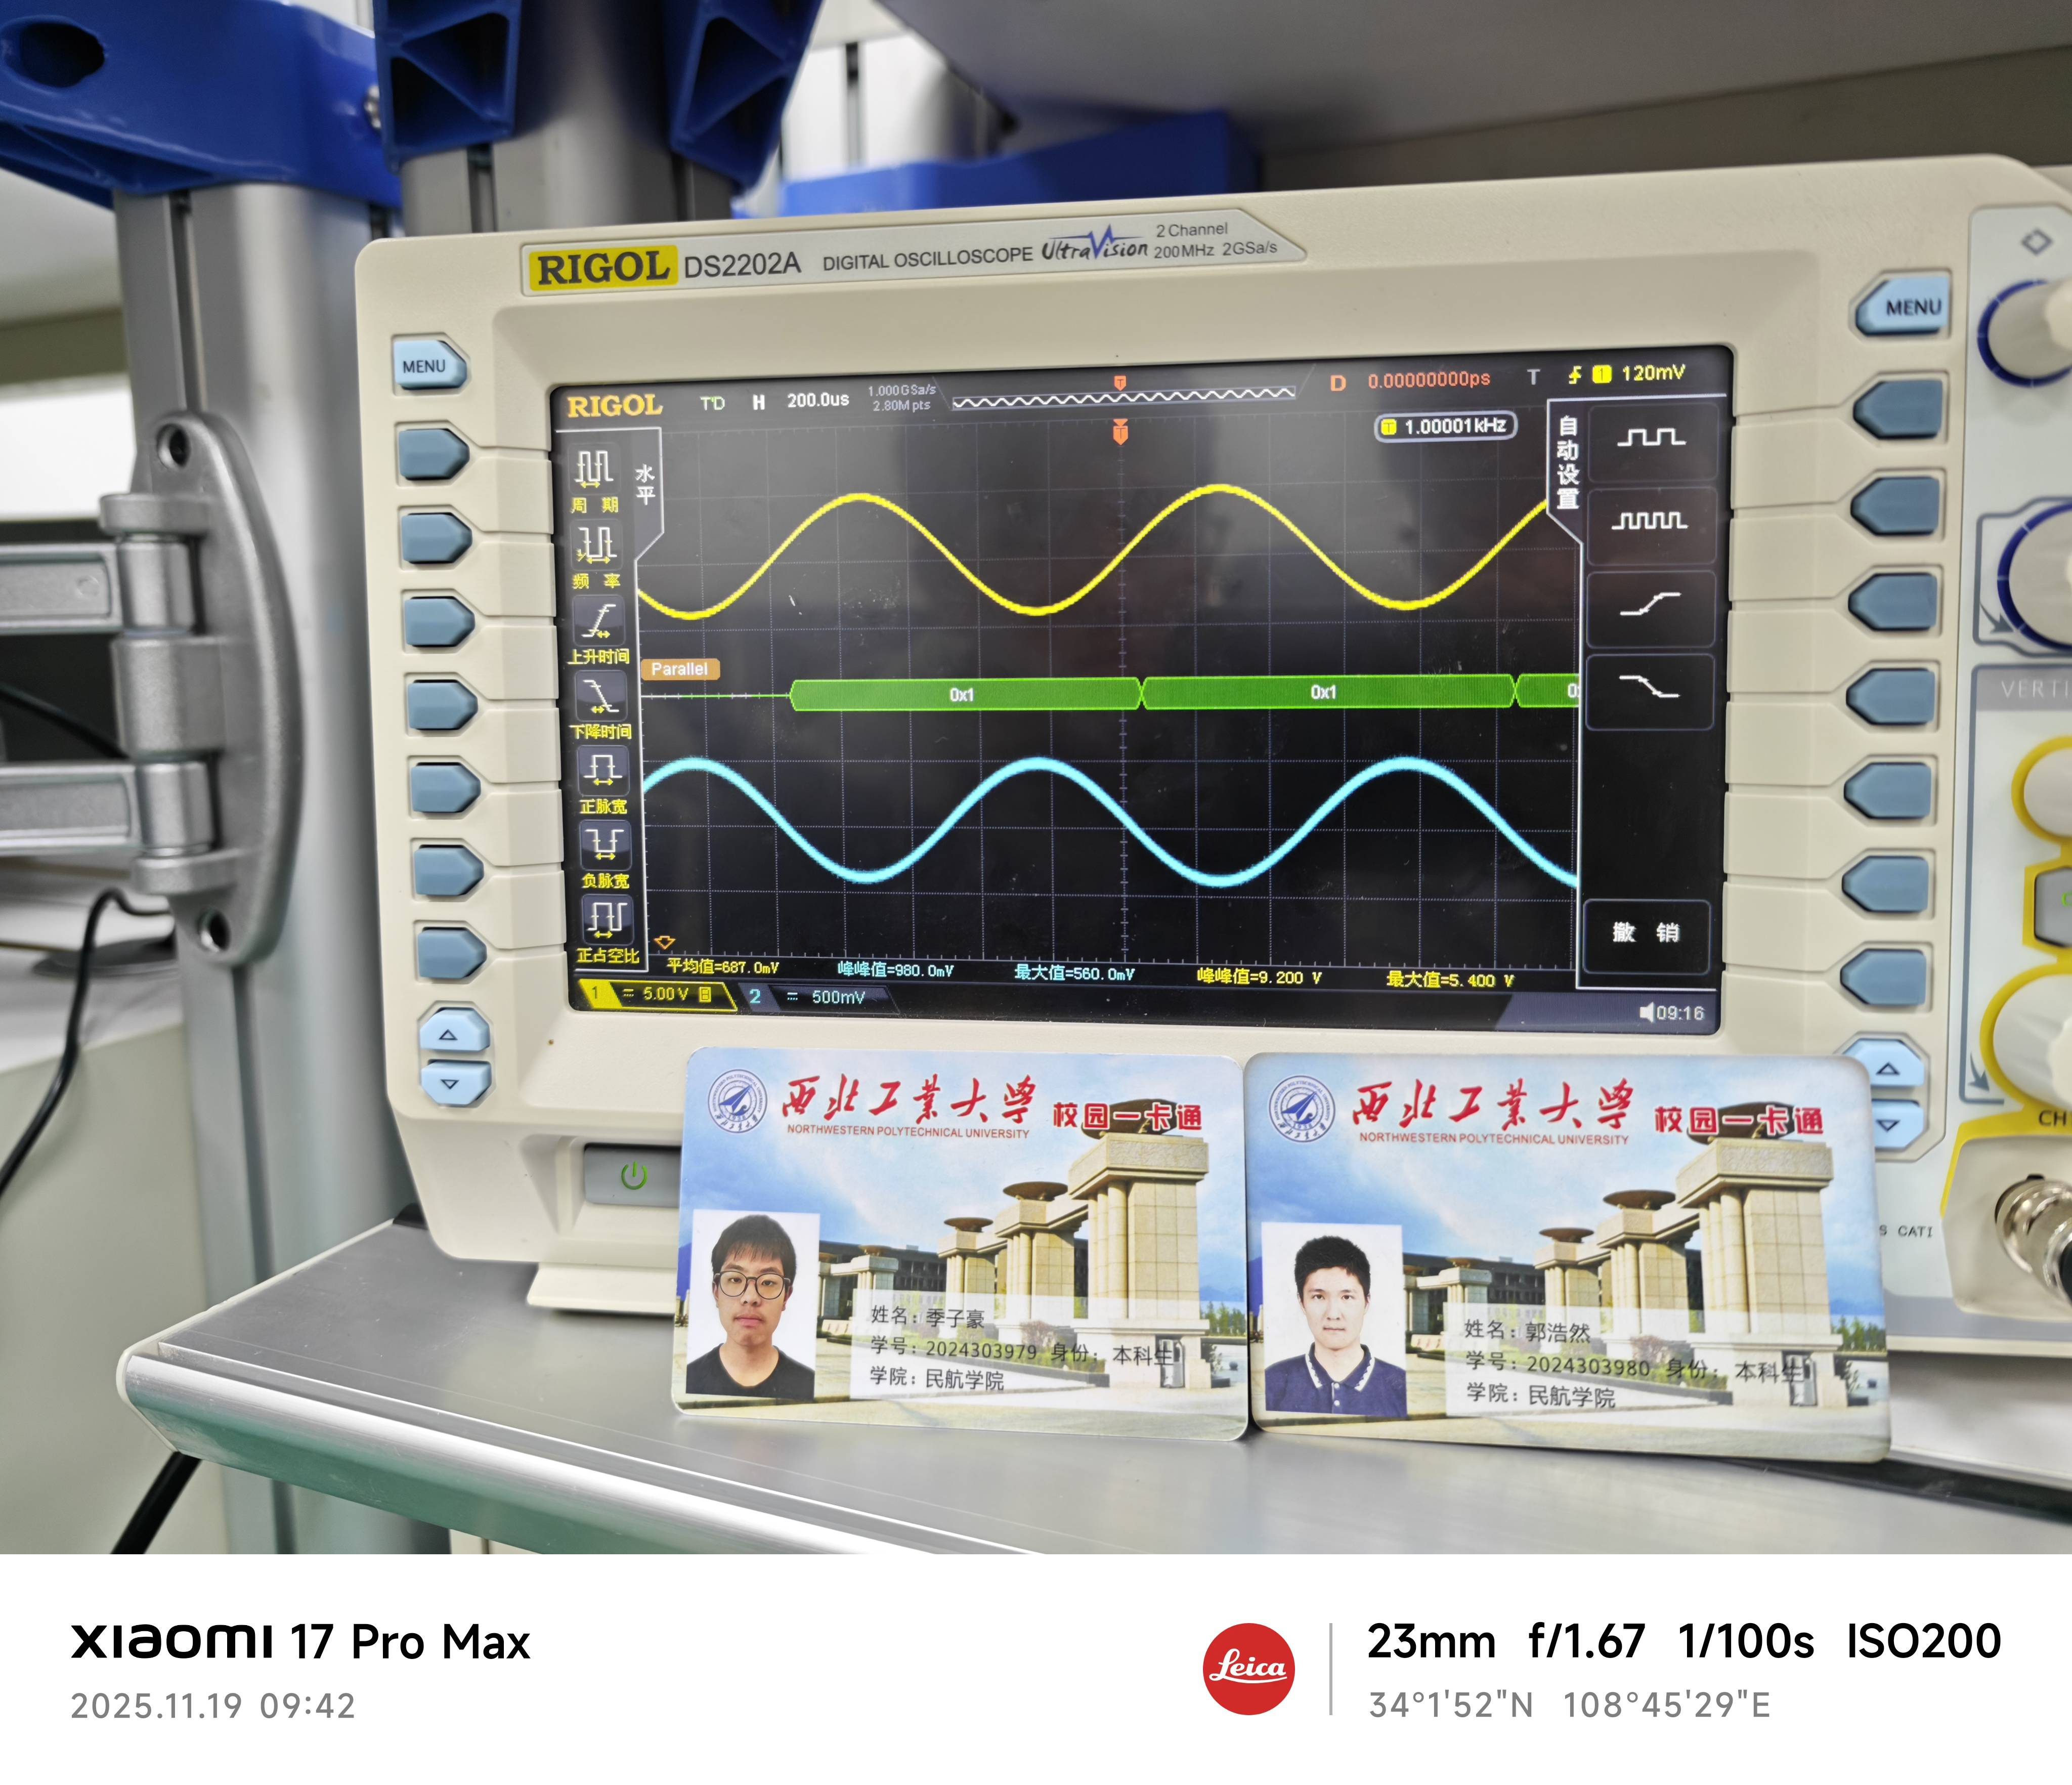
\includegraphics[width=\textwidth]{figures/比例器1.jpg}
        \caption{第二组电阻 ($R_2 = \SI{10}{\kilo\ohm}$)}
    \end{subfigure}
    \caption{比例放大器输入输出波形}
    \label{fig:result-prop}
\end{figure}

\subsubsection{积分器}
输入信号为 $f = \SI{1}{\kilo\hertz}$ 的方波时，记录数据如表\ref{tab:int-data}所示。输入输出信号波形图如图\ref{fig:result-int}所示。

\begin{figure}[H]
    \centering
    % --- 左侧：表格 ---
    \begin{minipage}[c]{0.48\textwidth}
        \centering
        \captionof{table}{积分器测试数据}
        \label{tab:int-data}
        % 使用 \small 稍微缩小字号以防表格宽度溢出半栏
        \small
        \begin{tabular}{ccc}
            \toprule
            电路参数 & \makecell[c]{输入 $V_{pp}$ \\ (\si{\volt})} & \makecell[c]{输出 $V_{pp}$ \\ (\si{\milli\volt})} \\
            \midrule
            \makecell[c]{$R_1 = \SI{1}{\kilo\ohm}$ \\ $R_2 = \SI{20}{\kilo\ohm}$} & 3.040 & 860.0 \\
            \bottomrule
        \end{tabular}
    \end{minipage}
    \hfill
    % --- 右侧：图片 ---
    \begin{minipage}[c]{0.48\textwidth}
        \centering
        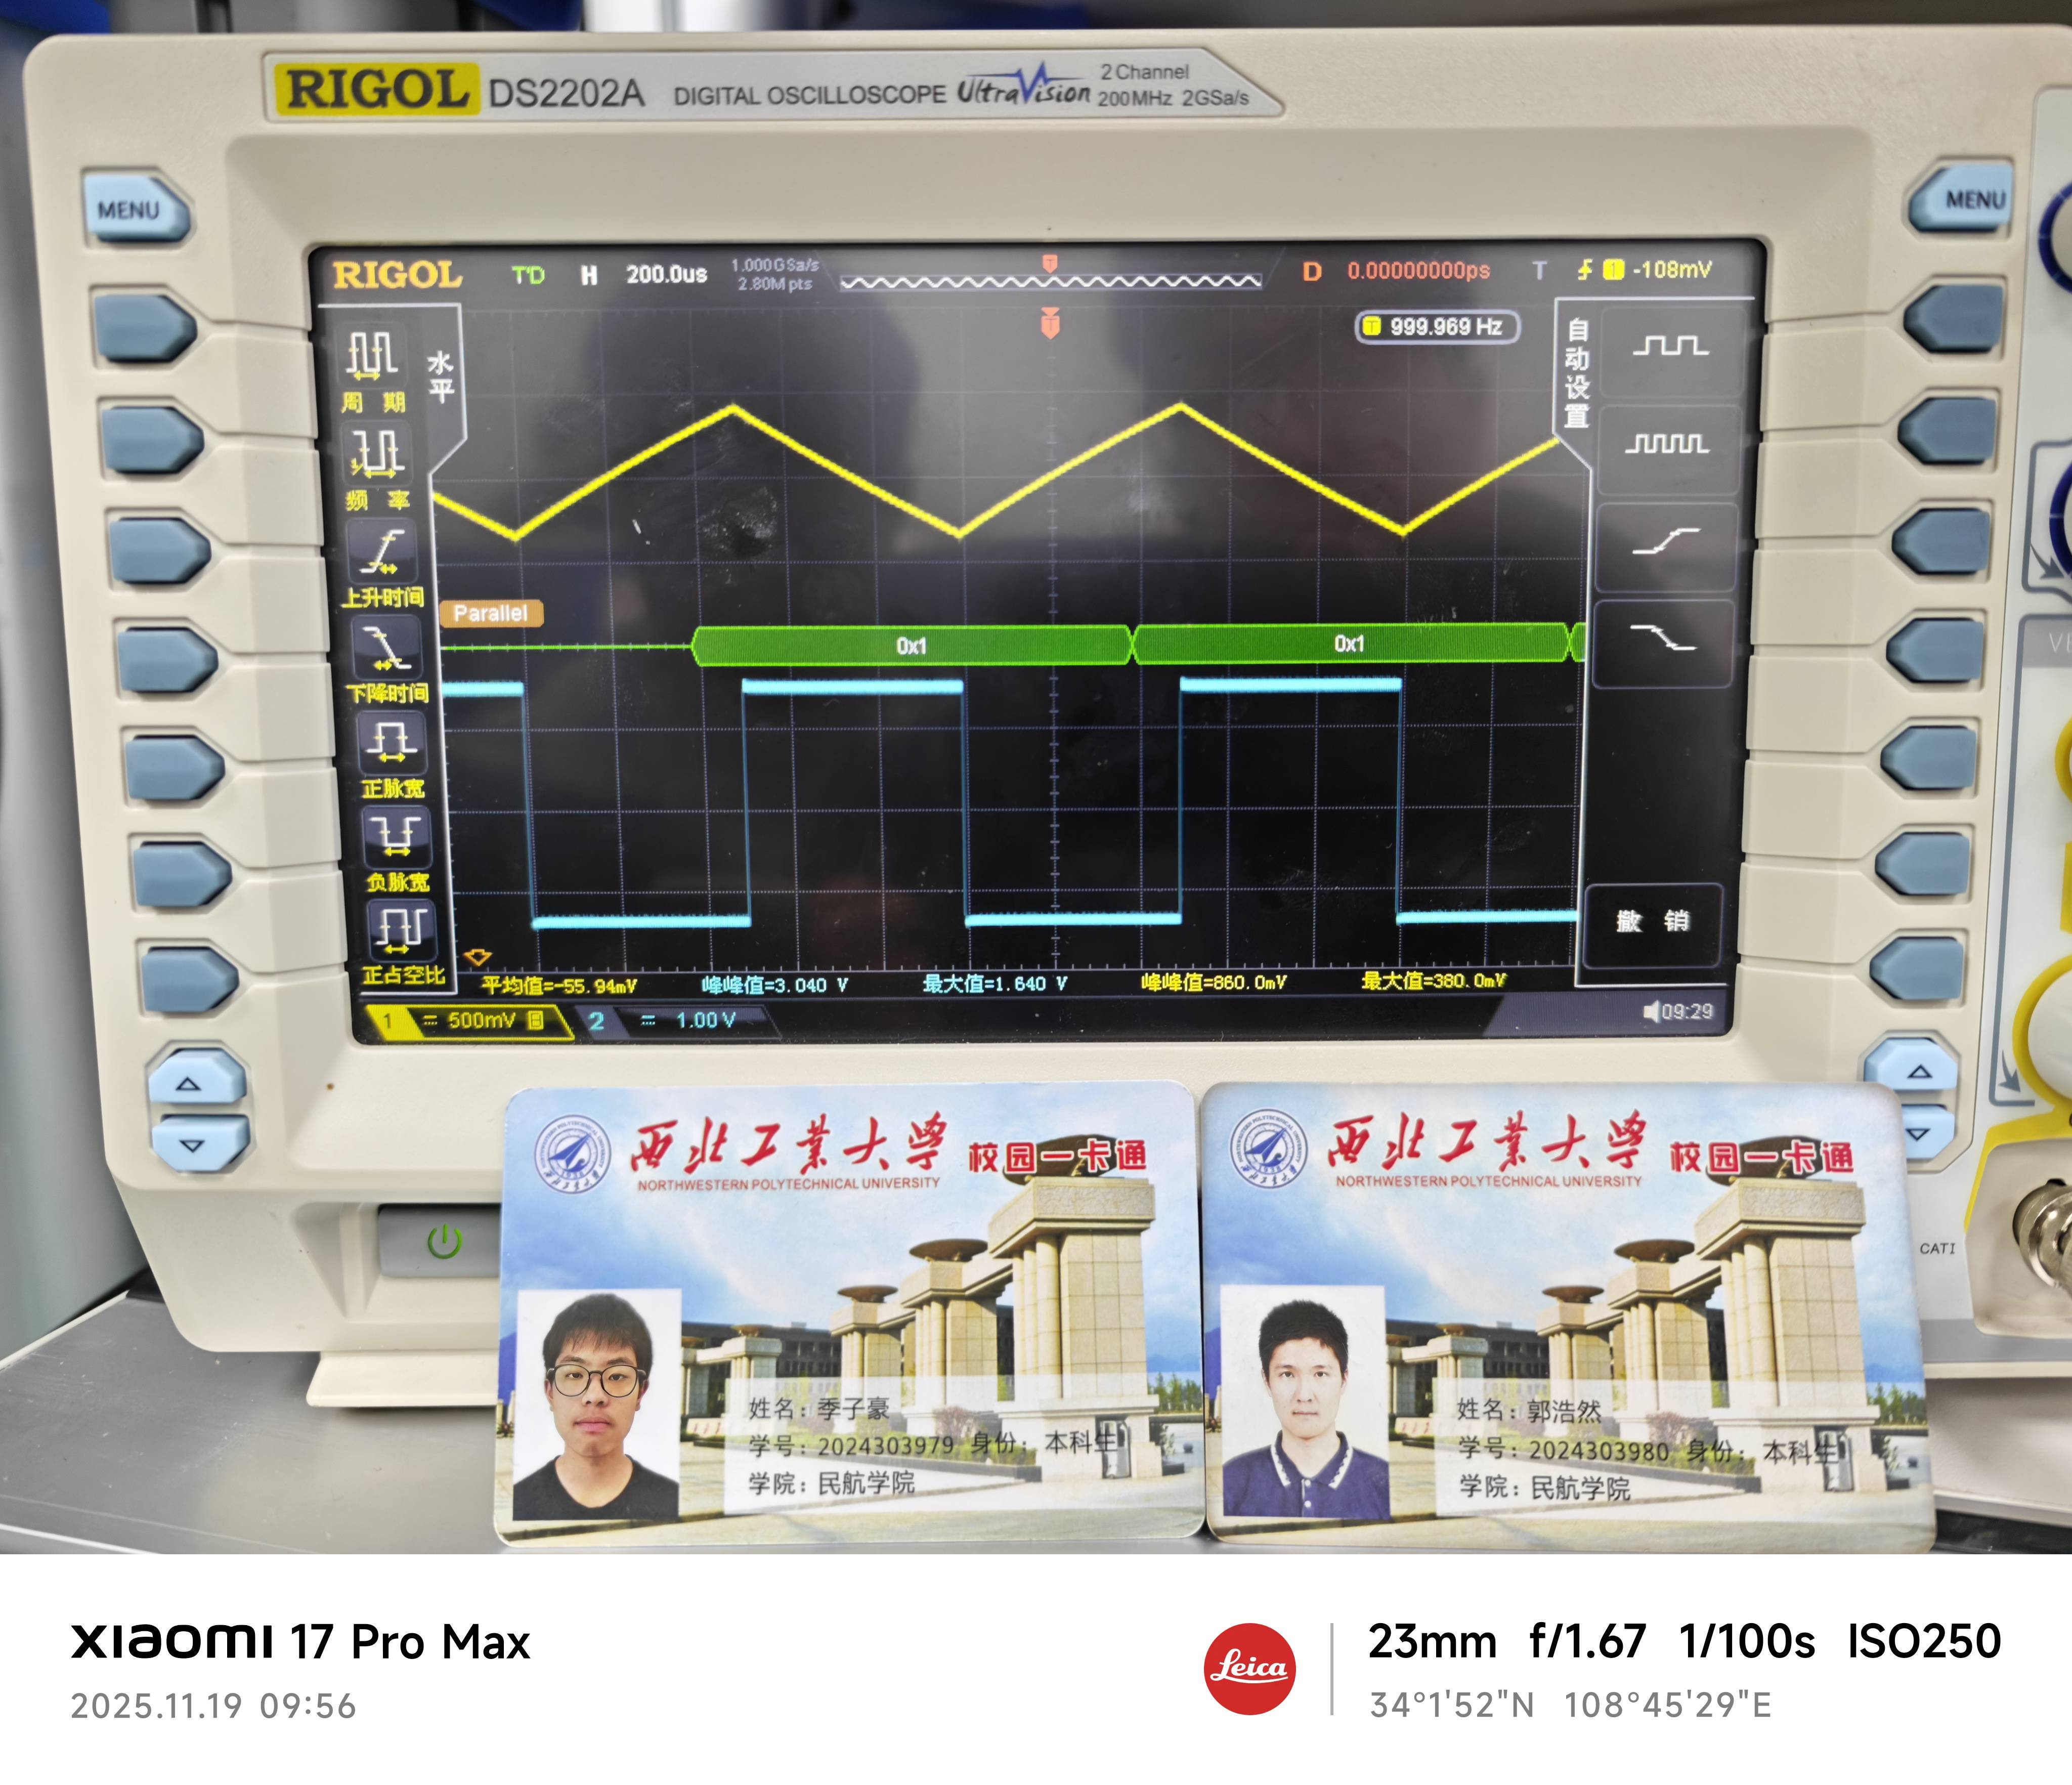
\includegraphics[width=\linewidth]{figures/积分器.jpg}
        \caption{积分器输入输出波形（方波输入）}
        \label{fig:result-int}
    \end{minipage}
\end{figure}

\subsection{一阶模拟电路阶跃响应}
当输入为幅度 \SI{1}{\volt}、频率 \SI{1}{\kilo\hertz} 的方波（可近似为周期性阶跃信号）时，一阶RC模拟电路的输出电压波形如图\ref{fig:result-rc}所示，呈现出典型的RC电路充放电曲线。

\begin{figure}[H]
    \centering
    % --- 左侧：表格 ---
    % 虽然原文是先图后表，但为了排版整齐，建议统一为左表右图
    \begin{minipage}[c]{0.48\textwidth}
        \centering
        \captionof{table}{一阶模拟电路阶跃响应参数记录}
        \label{tab:rc-params}
        % 表格内容较少，通常可以直接放下
        \begin{tabular}{lcc}
            \toprule
            测量对象 & \makecell[c]{$V_{pp}$ \\ (\si{\volt})} & \makecell[c]{$f$ \\ (\si{\kilo\hertz})} \\
            \midrule
            输入信号 & 2.0 & 1.0 \\
            输出信号 & 1.63 & 1.0 \\
            \bottomrule
        \end{tabular}
    \end{minipage}
    \hfill
    % --- 右侧：图片 ---
    \begin{minipage}[c]{0.48\textwidth}
        \centering
        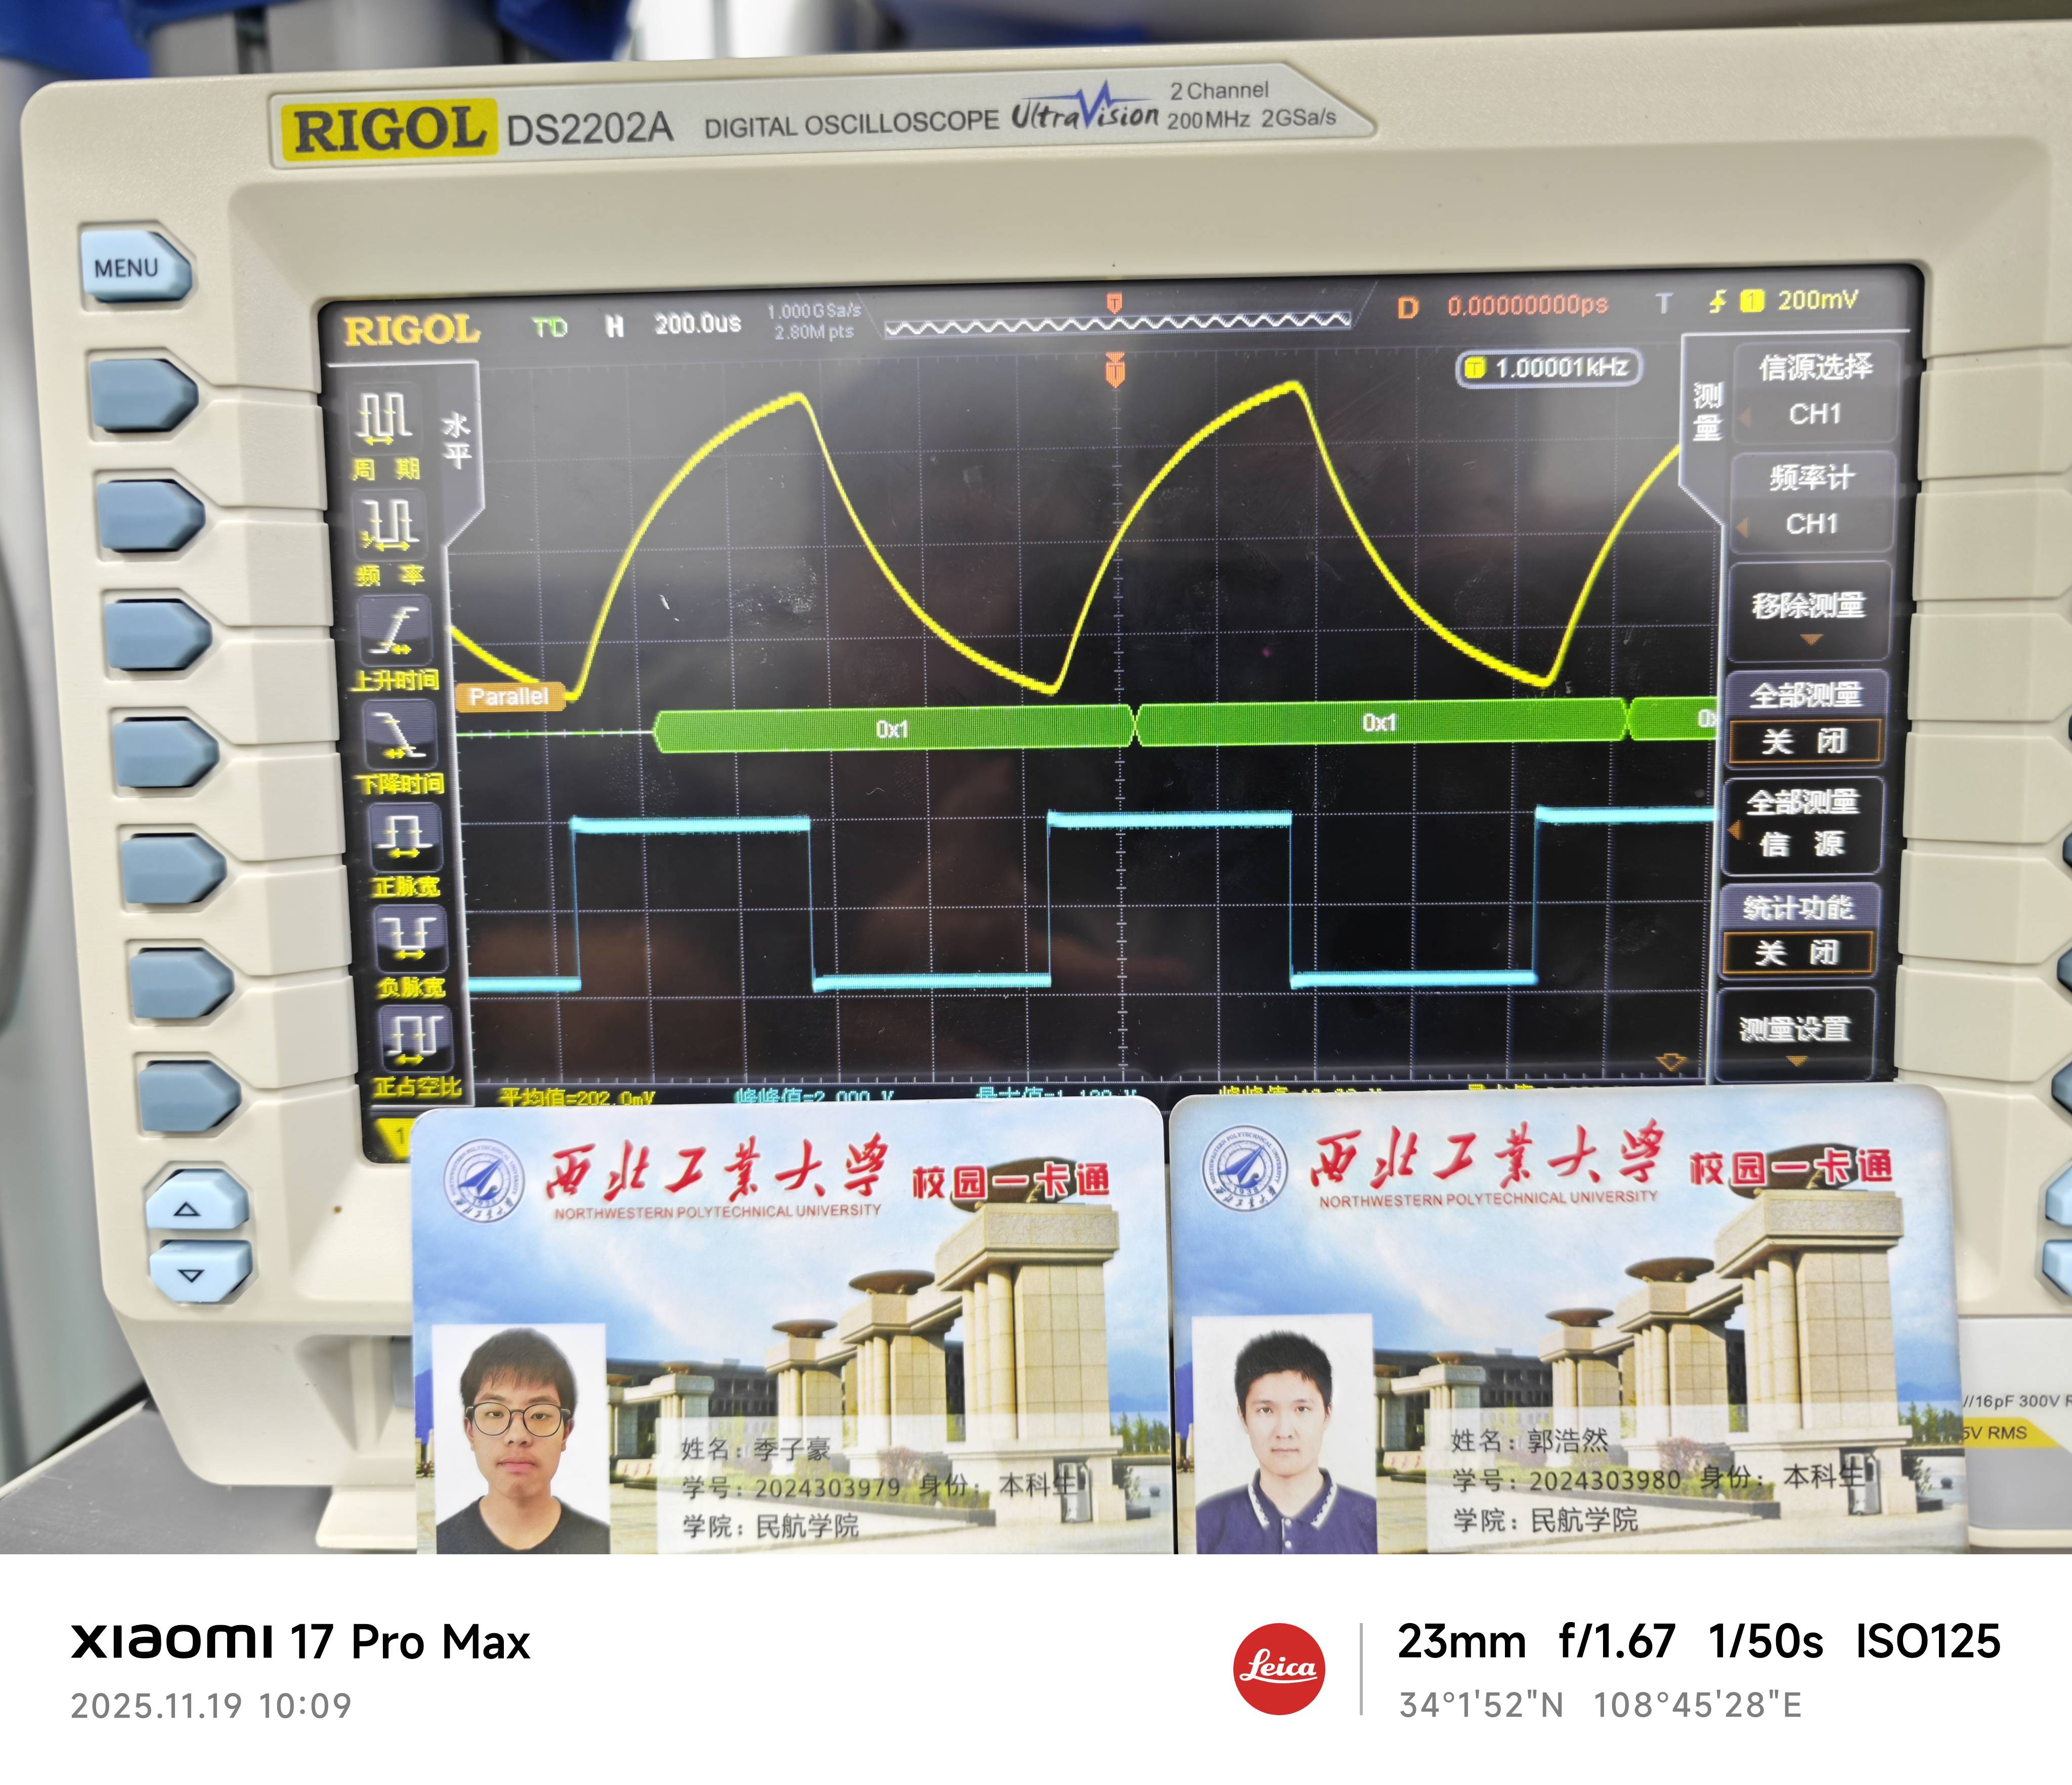
\includegraphics[width=\linewidth]{figures/系统模拟.jpg}
        \caption{一阶RC电路模拟输出波形}
        \label{fig:result-rc}
    \end{minipage}
\end{figure}

\section{实验结论}
% 以下是结论内容的示例，请根据您的实际情况进行修改。
\begin{enumerate}
    \item 通过本次实验，我深入了解了比例放大器、加法器和积分器这三种基本运算单元的电路结构与实际运算功能。实验结果表明，加法器能够实现多路信号的代数和（反相），比例放大器的放大倍数由反馈电阻与输入电阻之比决定，积分器则能将方波输入转换为三角波输出，验证了其积分特性。
    
    \item 我掌握了使用基本运算单元搭建模拟电路的方法，并成功地运用加法器和积分器模拟了一阶RC电路的阶-跃响应。实验观测到的输出波形（如图\ref{fig:result-rc}所示）与理论上的指数充放电曲线高度吻合，直观地展示了通过模拟电路研究实际系统动态特性的可行性与有效性。
    
    \item 实验过程中也注意到，实际测量值与理论计算值存在微小的误差（例如比例放大器的放大倍数并非精确等于 $R_2/R_1$），这可能来源于运放器件的非理想特性、电阻元件的精度误差、导线电阻以及测量仪器的内部误差等因素。
\end{enumerate}

% ===================================================================
% 报告正文结束
% ===================================================================

% ===================================================================
% MATLAB 信号仿真部分
% 请将此部分代码粘贴到 `实验报告` 章节之后，`实验结论` 章节之前
% ===================================================================

\newpage

\section*{{\LARGE{附录}}  \\ MATLAB 信号仿真}

\addcontentsline{toc}{section}{附录: MATLAB 信号仿真}
\markboth{附录}{\normalsize MATLAB 信号仿真}

本部分包含使用 MATLAB 进行信号卷积运算的仿真练习。

\subsection{课堂验收}
\begin{enumerate}
    \item 已知信号 $f(t) = e^{-t}u(t)$ 和 $h(t) = t^2e^{-2t}u(t)$，求 $y(t) = f(t) * h(t)$，结果如图\ref{fig:conv1}所示。
    \item 已知两信号 $f_1(t) = u(t) - u(t-1)$ 和 $f_2(t) = u(t+1) - u(t)$，求 $g_3(t) = f_1(t) * f_2(t)$，结果如图\ref{fig:conv2}所示。

    \begin{figure}[H]
        \centering
        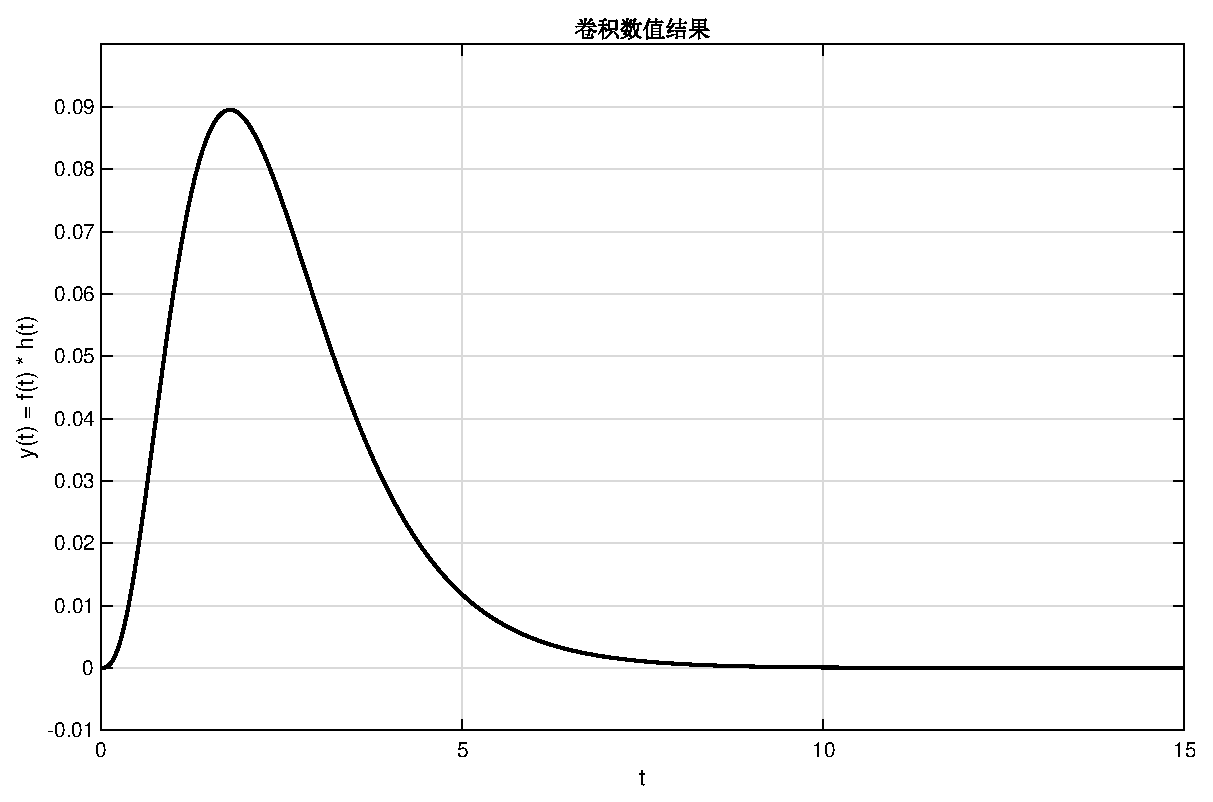
\includegraphics[width=0.6\textwidth]{figures/conv1.eps}
        \caption{信号 $f(t)=e^{-t}u(t)$ 与 $h(t)=t^2e^{-2t}u(t)$ 的卷积结果}
        \label{fig:conv1}
    \end{figure}
    
    
    \begin{figure}[H]
        \centering
        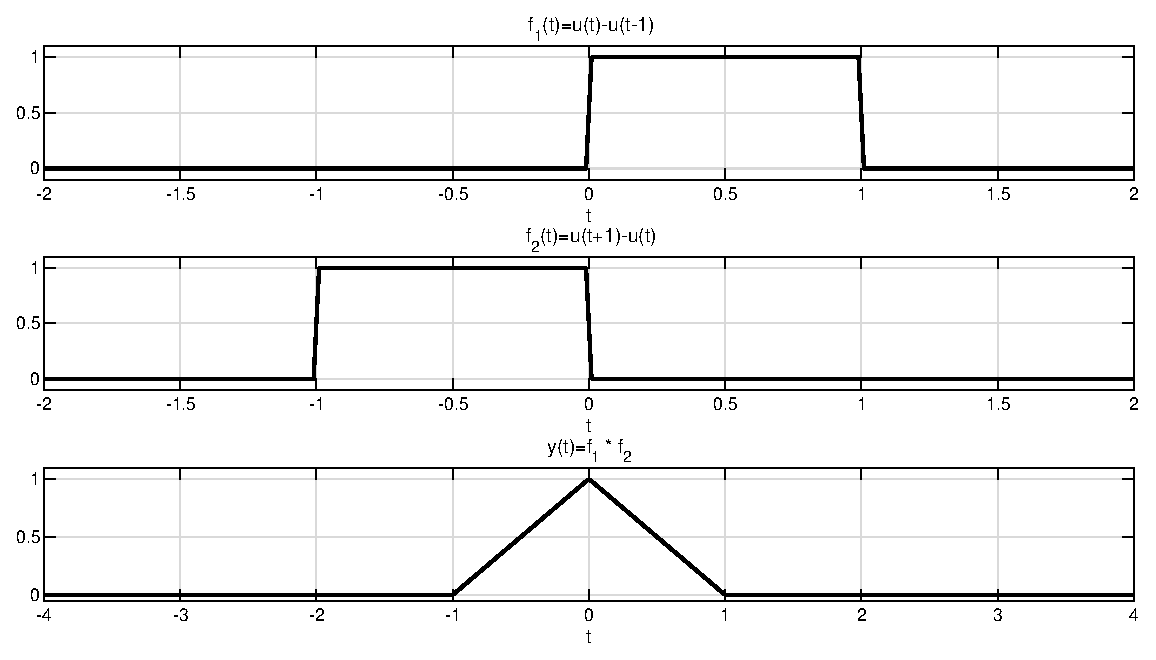
\includegraphics[width=0.6\textwidth]{figures/conv2.eps}
        \caption{信号 $f_1(t)=u(t)-u(t-1)$ 与 $f_2(t)=u(t+1)-u(t)$ 的卷积结果}
        \label{fig:conv2}
    \end{figure}
\end{enumerate}

\subsection{作业练习}
\begin{enumerate}
    \item 已知 $f_1(t) = u(t) - u(t-1)$, $f_2(t) = u(t+1) - u(t)$，求 $g_1(t) = f_1(t) * f_1(t)$, $g_2(t) = f_2(t) * f_2(t)$, $g_3(t) = f_1(t) * f_2(t)$。其中 $g_3(t)$ 的波形如图\ref{fig:homework}(a)所示。
    \item 对$f_1(t) = u(t-1) - u(t-2)$ 和 $f_2(t) = u(t) + u(t-1) - u(t-2) - u(t-3)$ 进行卷积，结果如图\ref{fig:homework}(b)所示。
    \item 对 $f_1(t) = u(t+1) - u(t-1)$ 和 $f_2(t)$进行卷积，结果如图\ref{fig:homework}(c)所示。
    \item 已知 $f_1(t) = (t-1)[u(t-1) - u(t-3)]$ 和 $f_2(t) = u(t+1) - 2u(t-2)$，求卷积，结果如图\ref{fig:homework}(d)所示。
\end{enumerate}

\begin{figure}[H]
    \centering
    \begin{subfigure}[b]{0.48\textwidth}
        \centering
        
\includegraphics[width=\textwidth]{figures/T1.eps}
        \caption{作业1结果}
    \end{subfigure}
    \hfill
    \begin{subfigure}[b]{0.48\textwidth}
        \centering
        
\includegraphics[width=\textwidth]{figures/T2.eps}
        \caption{作业2结果}
    \end{subfigure}
    
    \vspace{1em} % 增加垂直间距
    
    \begin{subfigure}[b]{0.48\textwidth}
        \centering
        
\includegraphics[width=\textwidth]{figures/T3.eps}
        \caption{作业3结果}
    \end{subfigure}
    \hfill
    \begin{subfigure}[b]{0.48\textwidth}
        \centering
        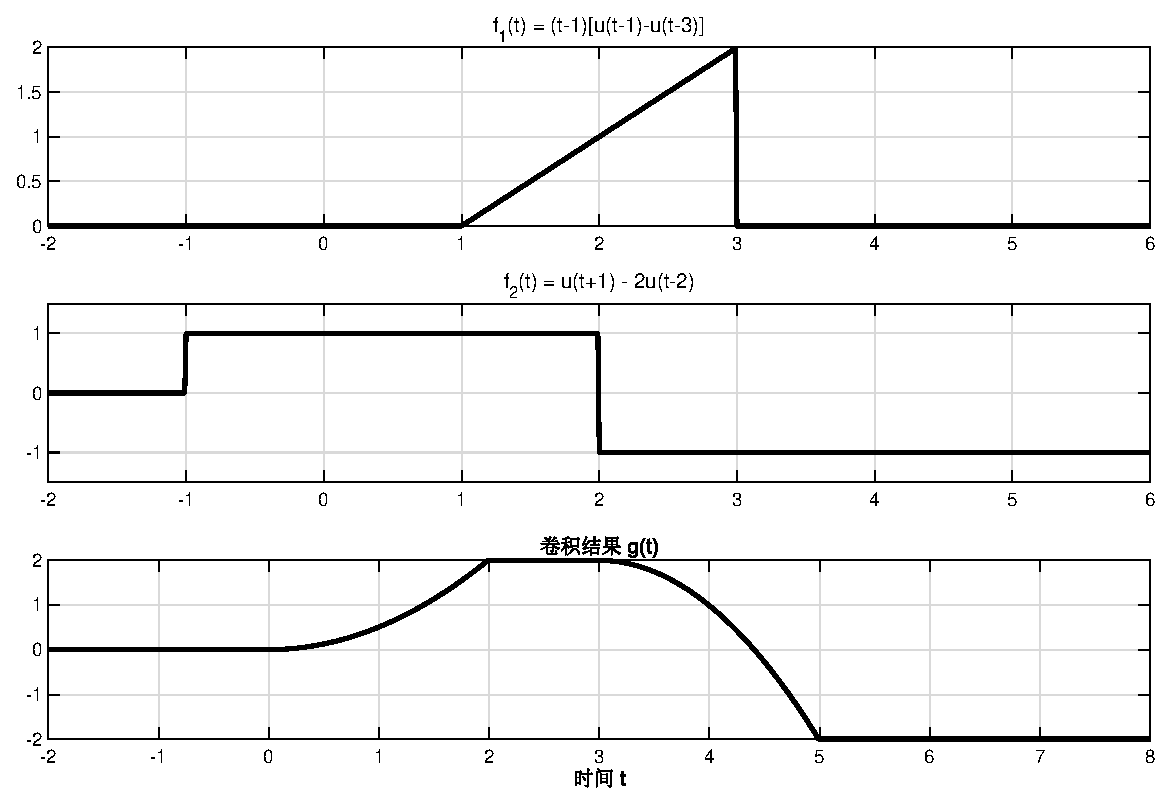
\includegraphics[width=\textwidth]{figures/T4.eps}
        \caption{作业4结果}
    \end{subfigure}
    \caption{MATLAB 作业练习卷积结果}
    \label{fig:homework}
\end{figure}

\newpage % 添加一个分页符，让结论部分在新的一页开始，版面更清晰

% ===================================================================
% MATLAB 仿真部分结束
% ===================================================================



\end{document}